\chapter{Experimental Apparatus}
\label{chap:experiment}

What machines must we build to examine the smallest pieces of the universe? The famous equation 
$E = m$ provides that to create massive particles, we need to provide enough energy. In order to give 
kinematic phase space to the types of processes that are examined in this thesis (and many others besides),
a system must be created in which there is enough energy to (at bare minimum), overcome kinematic thresholds:
if you want to search for $HH$ decays, you should have at least \SI{250}{\GeV} ($= 2\times m_{H}$) to work with.
It is not enough to simply induce such processes, however. These processes need to be captured in some way, emitted 
energy and particles must be characterized and identified, and in the end all of this information must be put into a 
useful and useable form such that selections can be made, statistics can be run, and a meaningful statement 
can be made about the universe. In this chapter, we describe the machines behind the physics, namely the Large 
Hadron Collider and the ATLAS experiment.

\section{The Large Hadron Collider}


\section{The ATLAS Experiment}

\section{}
\todo{Straight template copy}

% Footnote with ATLAS coordinate system
\newcommand{\AtlasCoordFootnote}{%
ATLAS uses a right-handed coordinate system with its origin at the nominal interaction point (IP)
in the centre of the detector and the \(z\)-axis along the beam pipe.
The \(x\)-axis points from the IP to the centre of the LHC ring,
and the \(y\)-axis points upwards.
Cylindrical coordinates \((r,\phi)\) are used in the transverse plane, 
\(\phi\) being the azimuthal angle around the \(z\)-axis.
The pseudorapidity is defined in terms of the polar angle \(\theta\) as \(\eta = -\ln \tan(\theta/2)\).
Angular distance is measured in units of \(\Delta R \equiv \sqrt{(\Delta\eta)^{2} + (\Delta\phi)^{2}}\).}


\begin{figure}[ht]
\centering
\subfloat{\label{fig:ATLAS-det}
		  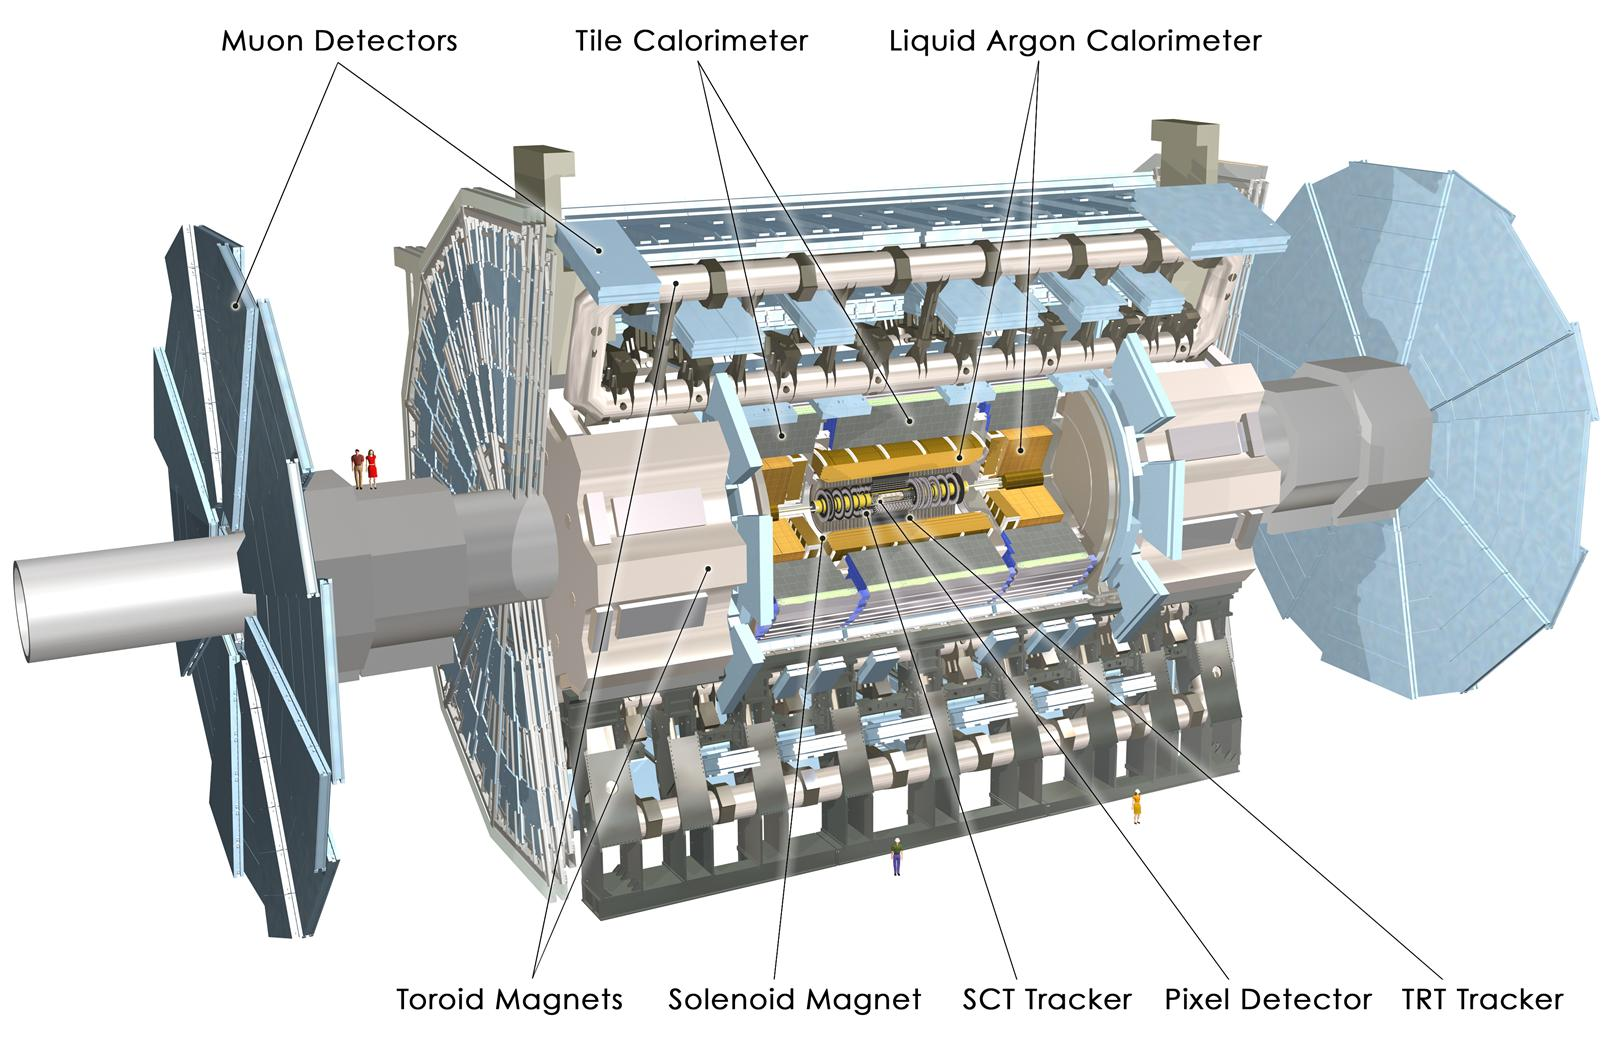
\includegraphics[width=0.8\textwidth]{figures/ATLAS-det.jpeg}
		 }
\caption{Diagram of the ATLAS detector \cite{DetectorImage}}
\end{figure}

\begin{figure}[ht]
\centering
\subfloat{\label{fig:ATLAS-shower}
		  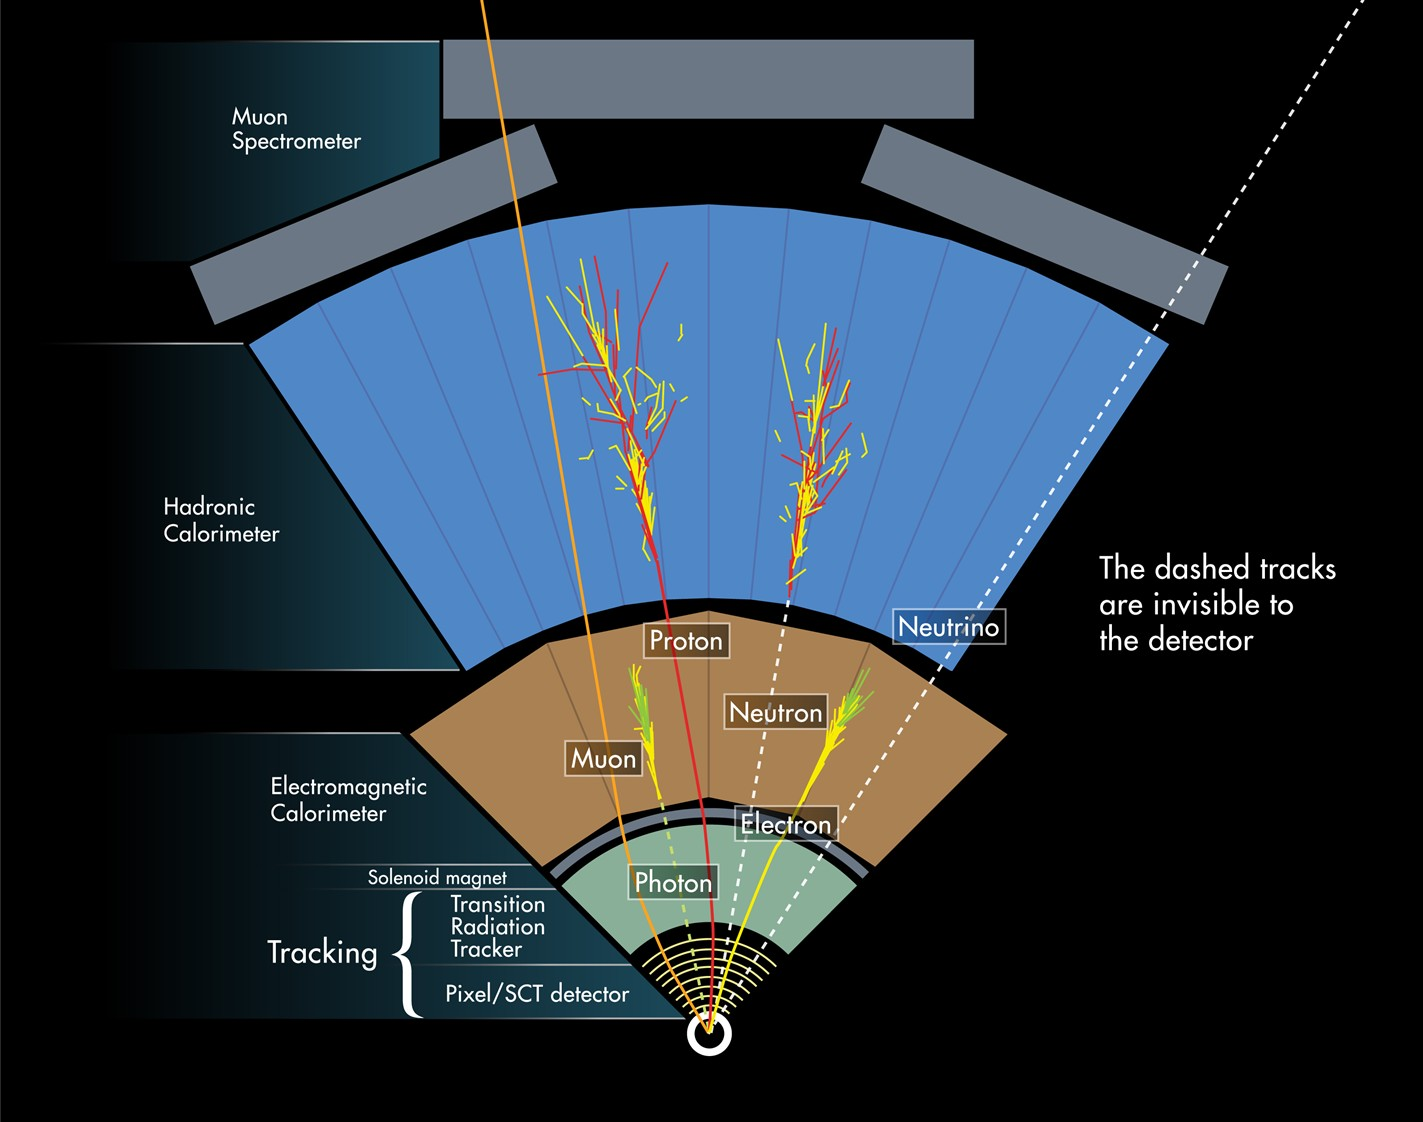
\includegraphics[width=0.8\textwidth]{figures/ATLAS-shower.jpeg}
		 }
\caption{Cross section of the ATLAS detector showing how particles interact with various detector components \cite{ShowerImage}}
\end{figure}

The ATLAS detector~\cite{PERF-2007-01} at the LHC covers nearly the entire solid angle around the collision point.\footnote{\AtlasCoordFootnote}
It consists of an inner tracking detector surrounded by a thin superconducting solenoid, electromagnetic and hadron calorimeters,
and a muon spectrometer incorporating three large superconducting air-core toroidal magnets.

The inner-detector system (ID) is immersed in a \SI{2}{\tesla} axial magnetic field 
and provides charged-particle tracking in the range \(|\eta| < 2.5\).
The high-granularity silicon pixel detector covers the vertex region and typically provides four measurements per track, 
the first hit normally being in the insertable B-layer (IBL) installed before Run~2~\cite{ATLAS-TDR-19,PIX-2018-001}.
It is followed by the silicon microstrip tracker (SCT), which usually provides eight measurements per track.
These silicon detectors are complemented by the transition radiation tracker (TRT),
which enables radially extended track reconstruction up to \(|\eta| = 2.0\). 
The TRT also provides electron identification information 
based on the fraction of hits (typically 30 in total) above a higher energy-deposit threshold corresponding to transition radiation.

The calorimeter system covers the pseudorapidity range \(|\eta| < 4.9\).
Within the region \(|\eta|< 3.2\), electromagnetic calorimetry is provided by barrel and 
endcap high-granularity lead/liquid-argon (LAr) calorimeters,
with an additional thin LAr presampler covering \(|\eta| < 1.8\)
to correct for energy loss in material upstream of the calorimeters.
Hadron calorimetry is provided by the steel/scintillator-tile calorimeter,
segmented into three barrel structures within \(|\eta| < 1.7\), and two copper/LAr hadron endcap calorimeters.
The solid angle coverage is completed with forward copper/LAr and tungsten/LAr calorimeter modules
optimised for electromagnetic and hadronic energy measurements respectively.

The muon spectrometer (MS) comprises separate trigger and
high-precision tracking chambers measuring the deflection of muons in a magnetic field generated by the superconducting air-core toroidal magnets.
The field integral of the toroids ranges between \num{2.0} and \SI{6.0}{\tesla\metre}
across most of the detector. 
A set of precision chambers covers the region \(|\eta| < 2.7\) with three layers of monitored drift tubes,
complemented by cathode-strip chambers in the forward region, where the background is highest.
The muon trigger system covers the range \(|\eta| < 2.4\) with resistive-plate chambers in the barrel, and thin-gap chambers in the endcap regions.

Interesting events are selected by the first-level trigger system implemented in custom hardware,
followed by selections made by algorithms implemented in software in the high-level trigger~\cite{TRIG-2016-01}. 
The first-level trigger accepts events from the \SI{40}{\MHz} bunch crossings at a rate below \SI{100}{\kHz},
which the high-level trigger further reduces in order to record events to disk at about \SI{1}{\kHz}.

An extensive software suite~\cite{ATL-SOFT-PUB-2021-001} is used for real and simulated data reconstruction
and analysis, for operation and in the trigger and data acquisition systems of the experiment.
